\documentclass[11pt]{article}
\usepackage[margin=1in]{geometry}
\usepackage[utf8]{inputenc}
\usepackage{amsmath}
\usepackage{graphicx}
\graphicspath{{./}{../paper/}}
\usepackage{xr}
\externaldocument[M-]{draft}
\renewcommand{\thesection}{S\arabic{section}}
\renewcommand{\thetable}{S\arabic{table}}
\renewcommand{\thefigure}{S\arabic{figure}}

\title{Supplementary Material for ``Levers and limits of active control in cross-situational word learning''}
\author{Shohei Hidaka, Takuma Torii, and George Kachergis}
\date{}

\begin{document}
\maketitle
\sloppy

This supplement gives implementation details and the mechanism and robustness analyses summarized in the main text. Section, table, and figure numbers beginning with S refer to this document; all others refer to the main text. Code and results are in the project repository (\texttt{corpusXSL/analysis}).

\section{Implementation and validation}
\label{sec-impl}
The reference implementations of both learners are written in R. For the eliminative learner, whose cost per episode grows with both $W$ and $C$, simulations at $C=100$, at $W \ge 10{,}000$, of the target-selection variants of Study 2, and of the ramps of Study 3 used a reimplementation in C++ with the same context construction and learning criterion but more efficient bookkeeping: weighted draws use a binary indexed tree rather than a linear scan, and each word's candidate referents are stored as a list rather than as a row of a $W \times W$ matrix. We validated it against the reference implementation on every condition both could complete: all four target $\times$ context conditions at $C=10$, familiar context at $C=100$, cross-word mutual exclusivity, each target-selection rule of Study 2, and every ramp and constant blend of Study 3. Mean episodes to 99\% agreed within sampling error ($|z| < 2$ in every comparison but one of the 29 in Study 3, a blend with $|z| = 2.5$), and adding the Study 2 options left results for the original conditions unchanged, seed for seed.

\section{Eliminative learner: unseen words dilute the familiarity signal}
\label{sec-dilution}
In Study 2, frequency-weighted choice sets were costly, and Goldilocks targeting helpful, only at $C=100$ with familiar context. Why should spreading exposures matter, and only there? Familiar-context selection weights each candidate distractor $r$ by $1/(n_r+1)$, where $n_r$ is the number of words that still hold $r$ as a possible meaning. A word that has never been the target of an episode has eliminated nothing, so it still holds every referent as a possible meaning, and each such unseen word adds the same amount to every referent's $n_r$. While many words are unseen, this shared count swamps the differences between referents, and familiar-context selection behaves almost like random selection. On this account, familiar context only starts to help once most words have been encountered at least once, and policies that concentrate targets on frequent words delay that point.

We tested this account in two ways, both at $C=100$, $a=1$ with familiar context (Table~\ref{tab-dilution}, Figure~\ref{fig-dilution}). First, we removed the dilution by computing each referent's familiarity from encountered words only, i.e.\ discounting the contribution of unseen words. If dilution is the mechanism, this should largely remove the differences between policies, and it does. The frequency-weighted choice set of 100 words goes from 5.7 times slower than unrestricted choice to 1.3 times; Goldilocks targeting goes from 0.57 to 0.93. At the 50\% checkpoint, the choice-set cost disappears entirely (5,547 episodes vs.\ 5,127 unrestricted, down from 84,671). What remains for small frequency-weighted choice sets (3.3x for 20 words) arises late in learning, and reflects the separate, direct problem that rare words are seldom in the choice set and so are seldom targeted. Removing the dilution also halves learning time for unrestricted active selection (15,770 to 7,803 episodes), while leaving passive sampling essentially unchanged (466,339 to 451,567), whose bottleneck is instead how rarely its rare words are targeted.

Second, we tracked each policy's trajectory under the original weighting. The frequency-weighted choice set leaves many words unencountered for a long time--634 after 10,000 episodes, against 63 for unrestricted choice and 34 for a uniform choice set--and throughout this period, 96--98\% of a target's remaining competing referents reappear among its distractors, escaping elimination, against 66--84\% for the other policies. Goldilocks targeting, which favors words encountered only once or twice, brings the number of unencountered words down fastest (33 after 5,000 episodes) and has the lowest competitor survival (about 50\%).

\begin{table}[h]
\centering
\caption{\label{tab-dilution} Episodes to learn 99\% of a $W=1{,}000$-word Zipfian ($a=1$) vocabulary at $C=100$ with familiar context, relative to unrestricted active selection under the same familiarity measure (30 replications per cell). ``All words'': the original familiarity measure, in which every unencountered word counts as still holding every referent; ``encountered words only'': that contribution removed.}
\small
\begin{tabular}{lrr}
\hline
 & \multicolumn{2}{c}{Familiarity computed from} \\
Condition & All words & Encountered words only \\
\hline
Unrestricted active (episodes) & 15{,}770 & 7{,}803 \\
\hline
Choice set of 100, frequency-weighted & 5.66x & 1.34x \\
Choice set of 20, frequency-weighted & 11.2x & 3.32x \\
Choice set of 100, uniform & 0.96x & 1.01x \\
Goldilocks & 0.57x & 0.93x \\
Passive & 29.6x & 57.9x \\
\hline
\end{tabular}
\end{table}

\begin{figure}[h]
\begin{center}
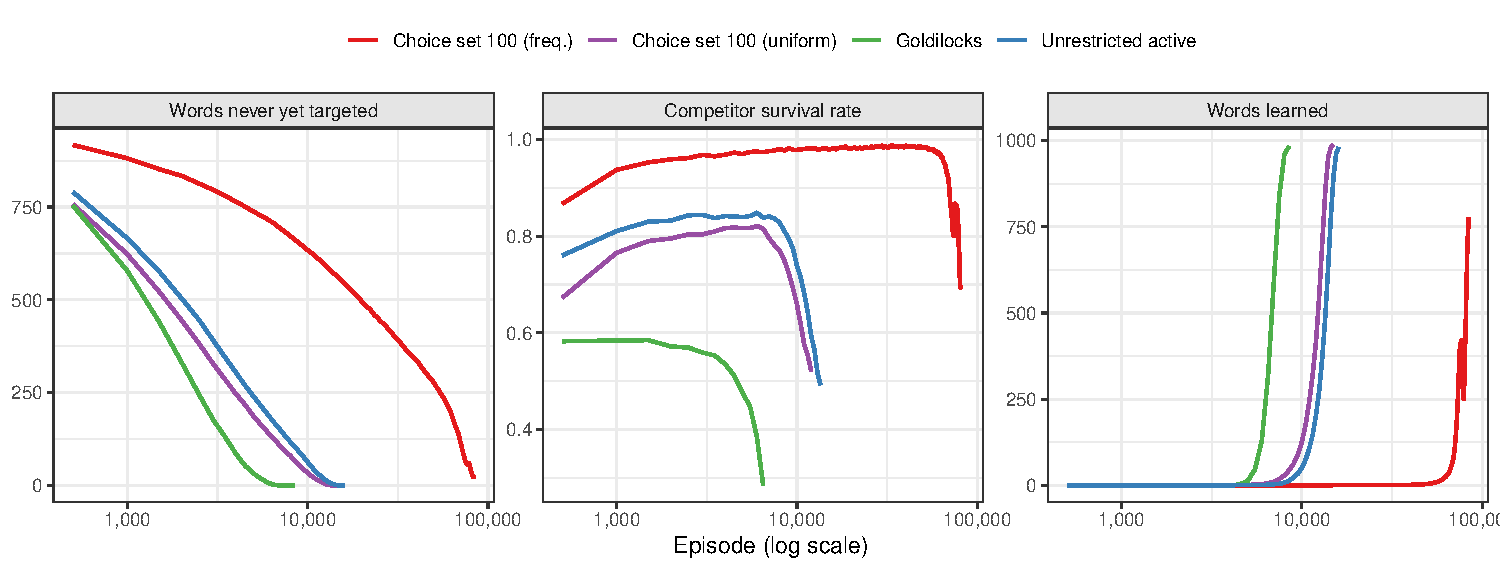
\includegraphics[width=\linewidth]{familiar_dilution.pdf}
\caption{\label{fig-dilution}
Trajectories under the original familiarity measure, $C=100$, $a=1$, familiar context (means of 10 runs). Left: words never yet targeted. Middle: competitor survival, the share of the target's remaining competing referents that reappear among its distractors and so escape elimination, shown until half the vocabulary is learned. Right: words learned. The frequency-weighted choice set leaves many words unencountered for longer, and while it does, familiar-context selection barely reduces competitor survival.}
\end{center}
\end{figure}

Why only at large $C$? At $C=10$ elimination is fast even with random distractors, so familiar-context selection adds relatively little (Study 1 of the main text finds a 2-fold benefit at $C=10$, against a difference between learning and not learning at all at $C=100$), and a policy that delays its benefit loses correspondingly little.

These tests also suggest a modeling point. The dilution arises from treating a never-encountered word as ``still considering every referent'', which is the natural bookkeeping for an eliminative learner, but not the only plausible one: a learner that simply ignores words it has not yet heard when judging how familiar an object is learns twice as fast under unrestricted active selection, and is far less sensitive to how its choice set is composed.

\section{Eliminative learner: which unnamed object to pursue}
\label{sec-policy}
An active learner must also decide which of the objects it cannot yet name to pursue. Our default chooses in proportion to frequency, so that common objects are pursued more often than rare ones; a uniform policy ignores frequency. Table~\ref{tab-policy} compares the two for the eliminative learner (30 replications per cell, none censored).

\begin{table}[h]
\centering
\caption{\label{tab-policy} Mean episodes to learn 99\% of the vocabulary, eliminative learner, under frequency-weighted and uniform active target selection, and the corresponding speedups over passive selection in the same set of runs.}
\small
\resizebox{\linewidth}{!}{\begin{tabular}{lrrrrr}
\hline
 & \multicolumn{2}{c}{Active (episodes)} & & \multicolumn{2}{c}{Speedup over passive} \\
Setting & Freq.-weighted & Uniform & Passive & Freq.-weighted & Uniform \\
\hline
$W=1{,}000$, $C=10$, $a=1$, random & 4{,}657 & 4{,}670 & 88{,}220 & 18.9x & 18.9x \\
$W=10{,}000$, $C=10$, $a=1$, random & 34{,}499 & 34{,}487 & 836{,}037 & 24.2x & 24.2x \\
$W=1{,}000$, $C=100$, $a=0.75$, random & 632{,}415 & 631{,}345 & 6{,}843{,}752 & 10.8x & 10.8x \\
$W=1{,}000$, $C=10$, $a=1$, familiar & 3{,}123 & 2{,}893 & 45{,}355 & 14.5x & 15.7x \\
$W=1{,}000$, $C=100$, $a=1$, familiar & 15{,}978 & 8{,}181 & 474{,}823 & 29.7x & 58.0x \\
\hline
\end{tabular}}
\end{table}

With random context the policy makes no difference: the number of exposures a word needs does not depend on which other words are already known, so any learner that targets only unknown words takes about the total number of exposures needed, whatever their order. With familiar context the policy matters, slightly at $C=10$ (8\%) and greatly at $C=100$, where uniform targeting halves the learning time and roughly doubles the active advantage, from 30-fold to 58-fold. The reason is the dilution of the familiarity signal by words not yet heard (Section~\ref{sec-dilution}): after 5,000 episodes, frequency-weighted targeting had left 239 words unheard on average, uniform targeting about 6 (10 replications each). With that dilution removed, by computing familiarity from heard words only, frequency-weighted targeting reached 99\% in 7,698 episodes, close to uniform targeting (8,041). The active advantages reported for familiar context elsewhere in this paper use frequency-weighted targeting and are therefore conservative. For the guess-test learner, the policy matters even with random context (main text, Table~\ref{M-tab-modes-gt}): uniform targeting is about twice as fast at $C=10$ and four times as fast at $C=100$, although at $C=100$ with familiar context it fails, like frequency-weighted targeting.

\section{Guess-test learner: blocked words and self-confirming errors}
\label{sec-gt-mech}
To find out why the policies of Study 2 help or fail the guess-test learner, we reimplemented it with additional bookkeeping (\texttt{corpusXSL/analysis/diagnose\_guesstest.R}) and ran a small number of instrumented replications, with and without targeted interventions.

\textit{Blocked words.} For the guess-test learner, a word can be learned only when it is the target and its own referent is not held, as a wrong guess, by another word. At $C=100$ this is the norm rather than the exception: in instrumented runs with random context, 97.5--99.9\% of active episodes targeted an unknown word whose referent was held by another word. Such a word is learned only after the word holding its referent is itself targeted, in a context without that referent, and drops its guess. Learning speed therefore depends on how often the words holding others' referents are targeted.

\textit{Familiar context at $C=100$: errors that confirm themselves.} For the guess-test learner, familiar-context selection weights each referent by how often its word's current guess has been confirmed, and confirmations do not distinguish right guesses from wrong ones. In four of six instrumented fully active runs that had not finished after $10^6$ episodes, every one of the 12--17 remaining unknown words held a wrong guess on another unknown word's referent, so each word's own referent was held by another unknown word. A fully active learner never targets known words (and, as noted in the General method, stops targeting a word as soon as its guess is correct), so their confirmation counts stay at zero, while each surviving wrong guess raises the weight of its word's referent. By the end, more than 99.99\% of the familiarity weight lay on referents of unknown words. Contexts were then filled with exactly the referents these wrong guesses claimed, so the guesses were confirmed rather than disconfirmed, and the set of mutually wrong guesses sustained itself. Two interventions confirm this account. Spending a quarter of episodes rehearsing a known word, chosen by frequency, let all six runs finish, in 48,706--59,042 episodes--faster than passive (85,818) or partially active learning (68,658--80,128). Computing familiarity only from confirmations of known words, an oracle the learner does not have, also let all six runs finish (148,335--224,512 episodes). Passive episodes help because they mostly rehearse known, frequent words, raising the familiarity of their referents and diluting the self-confirming set. Goldilocks targeting fails in this setting because it, too, never targets known words.

\textit{Choice sets at $C=100$: frequency counted twice.} When the choice set is drawn in proportion to frequency, and the target is then chosen within it in proportion to frequency again, a word's chance of being targeted grows roughly with the square of its frequency. Estimating the effective exponent $b$ in $P(\mathrm{target}) \propto p^b$ by simulating the target-selection rule directly gives $b \approx 1$ for unrestricted choice and $b = 1.6$--1.9 for choice sets of 20--100 words while many words are unknown. Small sets rarely contain more than one unknown word once learning is under way, so for them $b$ falls back toward 1 (1.06 for a set of 5 with 100 words unknown, 1.25 for a set of 20), at the cost of episodes spent on known words when the set contains no unknown word. This explains why intermediate sets cost the most. Steep weighting is costly for the guess-test learner because of blocking: it keeps choosing frequent blocked words and seldom chooses the rarer words that block them. At the end of instrumented runs with sets of 50 or 100 words, blocked words had typically been targeted tens of thousands of times, and the words blocking them far less often, usually only tens of times. Keeping the frequency-weighted set but choosing uniformly within it removes the cost: with sets of 100 words, learning took 75,844--85,409 episodes instead of 1.6--1.7 million.

\textit{Spreading targets helps.} The same account explains the benefit of Goldilocks targeting, which avoids returning to words that have been targeted many times without success: at $C=10$, only 2--5\% of its active episodes targeted a word already targeted ten or more times, against 47--61\% for unrestricted active selection. Spreading targets uniformly over the unknown words helps about as much at $C=10$ and even more at $C=100$ with random context: it learned 99\% of the vocabulary in 3,760 episodes at $C=10$ and 43,144 at $C=100$, against 8,007 and 179,983 for frequency-weighted active selection (main text, Table~\ref{M-tab-modes-gt}). For this learner, then, frequency-weighted targeting--the default active policy throughout our work--is far from optimal, at least when the learner knows which of its guesses are correct: with a learning criterion the learner can observe, both policies leave many more runs stalled (Section~\ref{sec-lock}).

\section{Word-driven pursuit: fixation and the role of passive input}
\label{sec-wd}
\textit{Without passive input, word-driven pursuit can fixate.} At $C=100$, except with random context at $a=0.75$, fully word-driven learners usually did not finish, while passive and (for the eliminative learner with familiar context) object-driven learners did. None of the 30 eliminative runs with familiar context learned even 10\% of the vocabulary in $5 \times 10^8$ episodes. An instrumented run shows why. The first word it heard happened to be the most frequent word, the only word whose competitors do not include the most frequent referent, and it was learned after 10,144 exposures. Every other word must rule out that referent, which with frequency-weighted distractors is absent from a context with probability about $5 \times 10^{-10}$ (Study 1). The learner then pursued the second word it heard for the next two million episodes without learning it, never hearing a third. With 998 words unheard, the familiarity signal is almost entirely diluted, so distractors are effectively drawn by frequency, and every one of the target's competing referents reappeared in every context. A learner whose first word is any other word is stuck on that word from the start. The guess-test learner fixates differently: in five of six instrumented runs with random context, after $3 \times 10^5$ episodes the learner had heard a single word, whose wrong guess was the referent of the first- or second-most-frequent word--a referent almost never out of view, so the guess was almost never disconfirmed (\texttt{corpusXSL/analysis/diagnose\_word\_driven.R}). A passive learner falls into the same traps for individual words, but moves on; a word-driven learner with nothing new to hear cannot.

Passive episodes remove the fixation, because they supply new words to pursue (script \texttt{run\_word\_driven\_partial.R}; 30 replications per cell, none censored). Eliminative learners pursuing heard words on 25\%, 50\%, and 75\% of episodes, at $C=100$ with familiar context, finished in 52,582, 73,267, and 133,950 episodes, against 431,500 passive: more pursuit was slower, the opposite of the object-driven learner (28,723, 21,191, and 18,047 episodes at the same levels). Each word-driven episode is an episode not spent hearing a new word, and so prolongs the dilution of the familiarity signal. For the guess-test learner at $C=100$, partially word-driven learners did as well as partially object-driven ones (random context: 253,365, 215,625, and 182,398 episodes, against 255,740, 237,110, and 200,699; familiar context: 70,021, 68,911, and 85,905, against 68,658, 71,732, and 80,128), so here the cost of word-driven pursuit lies entirely in its failure without passive input.

\section{Guess-test learner with an observable learning criterion: Study 2}
\label{sec-lock}
As noted in the General method of the main text, the guess-test learner of Study 2 stops pursuing a word as soon as its guess is correct, which it cannot observe. We therefore reran its simulations with the lock-in criterion of Paper 1: a word is treated as known once its current guess has survived two consecutive exposures, and is scored as learned when that locked guess is also correct. Active selection pursues words whose guesses have not locked in. A locked wrong guess is still discarded if its word is heard without it, but an active learner never chooses such a word, so only passive episodes can correct it. There is no forgetting. We ran every condition of the main text's Table~\ref{M-tab-modes-gt}, fully word-driven targeting in all four settings, and word-driven pursuit on 25--75\% of episodes at $C=100$ (200 replications per cell at $C=10$, except 30 for word-driven targeting, and 30 at $C=100$; cap $5 \times 10^6$ episodes; \texttt{corpusXSL/analysis/run\_guesstest\_lock.R} and \texttt{run\_more\_reps.R}). Because runs that stall below 99\% dominate the means of some cells, Table~\ref{tab-lock} reports medians.

\begin{table}[h]
\centering
\caption{\label{tab-lock} Median episodes to learn 99\% of a $W=1{,}000$-word Zipfian ($a=1$) vocabulary, guess-test learner with an observable learning criterion (a word is known once its guess has been confirmed twice in a row; learned when that guess is also correct), 200 replications per cell at $C=10$ (word-driven: 30) and 30 at $C=100$. Numbers in parentheses: runs that did not finish within $5 \times 10^6$ episodes, counted at the cap; ``$>5 \times 10^6$'': more than half did not.}
\small
\begin{tabular}{lrrrr}
\hline
 & \multicolumn{2}{c}{$C=10$} & \multicolumn{2}{c}{$C=100$} \\
Condition & Random & Familiar & Random & Familiar \\
\hline
Passive & 56{,}140 & 47{,}086 & 296{,}828 & 102{,}112 \\
25\% active & 18{,}018 & 11{,}682 & 317{,}188 & 71{,}867 \\
50\% active & 15{,}652 & 8{,}768 & 340{,}749 & 74{,}995 \\
75\% active & 13{,}862 & 7{,}822 & 459{,}091 & 91{,}232 \\
Fully active & 12{,}714 (15) & 9{,}992 (1) & $>5 \times 10^6$ (30) & $>5 \times 10^6$ (30) \\
Goldilocks & 5{,}635 (71) & 4{,}838 (8) & $>5 \times 10^6$ (30) & $>5 \times 10^6$ (30) \\
Uniform & $>5 \times 10^6$ (132) & 5{,}388 (21) & $>5 \times 10^6$ (30) & $>5 \times 10^6$ (30) \\
Word-driven & $>5 \times 10^6$ (22) & $>5 \times 10^6$ (29) & $>5 \times 10^6$ (30) & $>5 \times 10^6$ (30) \\
Word-driven, 25\% & -- & -- & 276{,}445 & 70{,}535 \\
Word-driven, 50\% & -- & -- & 354{,}999 & 70{,}281 \\
Word-driven, 75\% & -- & -- & 417{,}500 & 104{,}657 \\
Choice set of 100 & 66{,}824 & 43{,}542 & $>5 \times 10^6$ (30) & $>5 \times 10^6$ (30) \\
Choice set of 50 & 60{,}323 & 40{,}329 & $>5 \times 10^6$ (30) & $>5 \times 10^6$ (30) \\
Choice set of 20 & 20{,}093 & 11{,}268 & $>5 \times 10^6$ (30) & 4{,}035{,}585 (9) \\
Choice set of 5 & 17{,}400 & 13{,}416 & 2{,}072{,}256 & 532{,}963 \\
\hline
\end{tabular}
\end{table}

\textit{At $C=10$ the active advantage survives.} Requiring confirmation slows passive learning (median 56,140 episodes with random context, against 38,176 with the original criterion) as well as active learning, and fully active learning remains 4.4 times faster than passive learning with random context (95\% CI 4.2--4.7) and 4.7 times with familiar context (4.4--5.1), by medians, against 5.0 (4.7--5.3) and 3.6 times (3.4--3.7) with the original criterion. With random context, 15 of 200 fully active runs stalled short of 99\%, as in Paper 1; with familiar context, 1 of 200 did.

\textit{At $C=100$, full control fails.} No learner choosing among all unnamed objects on every episode finished, with either kind of context and whether it chose by frequency, by Goldilocks preference, uniformly, or among heard words only, while every passive and partially active learner did. An instrumented reimplementation (\texttt{corpusXSL/analysis/diagnose\_lock\_stall.R}; six fully active runs per setting) found the same end state in all twelve runs. After $5 \times 10^5$ episodes the learner had learned 68--71\% of the vocabulary with random context and 78--81\% with familiar context, and every unlearned word but one held a locked wrong guess on the referent of another unlearned word. These were not only rare words: their median frequency rank was 195--222 with random context and 134--160 with familiar context. The one word not locked could not be learned, because its referent was held, and the words holding referents were never targeted again, because the learner believed it knew them. A locked wrong guess thus blocks the word whose referent it holds, and that word, unable to guess its own referent, eventually locks in a wrong guess of its own. With 100 referents in view, a wrong guess is far more often confirmed by chance, so the chain of blocked words takes in much of the vocabulary rather than a few words. In instrumented fully active runs with random context (six per context size), 0.7--0.9\% of wrong guesses survived two confirmations at $C=100$, against 0.03--0.13\% at $C=10$; by the time half the words had locked in a guess, 170--191 of these guesses were wrong at $C=100$, but only 1--4 at $C=10$. A passive episode can break the chain, by hearing a locked word in a context without its wrongly guessed referent. Bounded choice sets show the same thing: a small set often contains no unlocked word, and the learner then draws a word from the set by frequency, which may be a wrongly locked one. With sets of 5 words every run finished at $C=100$, and with sets of 20, 21 of 30 runs with familiar context did.

\textit{Partial control beats full control.} Every partially active learner finished. At $C=10$, being active on a quarter of episodes gained 77\% (random context; 95\% CI 73--80\%) and 90\% (familiar context; 86--94\%) of the full speedup on a log scale, by medians, more than with the original criterion (60\% and 99\% by means, 63\% and 98\% by medians). With familiar context, learners active on half or three-quarters of episodes were again faster than fully active ones (medians 8,768 and 7,822 episodes, against 9,992; CIs 8,578--8,950, 7,587--8,138, and 9,312--10,618). At $C=100$, partial control helped less than with the original criterion. With familiar context, learners active on a quarter or half of episodes were about 1.4 times faster than passive learners, but with random context partial control did not help at all (317,188--459,091 episodes, against 296,828 passive), whereas with the original criterion every partially active learner was faster than passive learning. Episodes spent pursuing unlocked words leave the wrongly locked words to be corrected by passive episodes alone.

\textit{Spreading targets speeds learning, at a price.} At $C=10$, Goldilocks targeting again roughly halved the median time of frequency-weighted active selection (5,635 vs.\ 12,714 episodes with random context, 4,838 vs.\ 9,992 with familiar context), and uniform targeting did the same with familiar context (5,388). But both left more runs stalled: Goldilocks targeting 71 and 8 of 200 (random and familiar context), uniform targeting 132 and 21, against 15 and 1 for frequency-weighted selection. With random context, every uniform run reached 90\% of the vocabulary, on average in 5,447 episodes, close to Goldilocks targeting (5,293) and half the time of frequency-weighted selection (10,894), but two-thirds of runs never reached 99\%. Spreading targets thus speeds the learning of most of the vocabulary but leaves more runs caught by errors they never revisit; we did not trace why.

\textit{Bounded choice is costlier.} With frequency-weighted choice sets, median times at $C=10$ were longer than with unrestricted choice for every set size (with random context, 17,400--66,824 episodes, against 12,714; with familiar context, 11,268--43,542, against 9,992), and at $C=100$ only sets of 5 words always finished.

\textit{Word-driven pursuit still depends on passive input.} Fully word-driven learners now failed even at $C=10$ (22 and 29 of 30 runs did not finish, against none with the original criterion). Pursuing heard words on 25--75\% of episodes at $C=100$, they did about as well as partially object-driven learners (random context: 276,445--417,500 episodes, against 317,188--459,091; familiar context: 70,281--104,657, against 71,867--91,232).

The observable criterion therefore leaves intact the active advantage at $C=10$, the value of partial control, and the dependence of word-driven pursuit on passive input, and it strengthens the conclusion that partial control can beat full control. It removes any benefit of full control at $C=100$, and it qualifies the benefit of spreading targets over the unknown words, which now comes with many more stalled runs.

\section{Observable learning criterion: Study 3}
\label{sec-lock-ramp}
With the observable learning criterion of Section~\ref{sec-lock} (the same ramps and blends as in Study 3 of the main text, 200 replications each; medians: passive 55,624 episodes, fully active 12,909), losing control early was again costly, but becoming active late no longer reliably helped. We matched ramps to blends on medians, because 20 of the 200 fully active constant runs stalled below 99\% and dominate the mean at high autonomy. Reverse ramps with $T \le 12{,}000$ were 1.2 to 2.3 times slower than matched blends, the cost growing with $T$ (every 95\% CI within $\pm 0.05$ of its estimate). The threshold again lies between $T=12{,}000$ and 20,000, but closer to 20,000 than with the original criterion: at $T=12{,}000$ the reverse ramp still took 50,956 episodes, near the passive level, and at $T=20{,}000$ it took 15,098 (1.10 times its matched blend, CI 1.02--1.25), as the $T/2$ rule predicts for this learner's slower active completion. Forward ramps were neither consistently faster nor slower than matched blends (ratios 0.85--1.04, with no trend in $T$; five of the seven CIs included 1, and the other two, at $T=3{,}000$ and 20,000, favored the ramp). Forward ramps stalled in 28 of 1,400 runs, mostly at the shortest timescales (15 of 200 at $T=1{,}000$, 4 and 7 at $T=2{,}000$ and 3,000, and at most 1 at $T \ge 5{,}000$), although every ramp ends fully active, which suggests that passive episodes early in learning protect against the chains of wrongly locked words described in Section~\ref{sec-lock}. A constant blend with 25\% active episodes captured 77\% (73--84\%) of the full speedup on a log scale, by medians.

\section{Observable learning criterion: Study 4}
\label{sec-lock-flickr}
With the observable learning criterion of Section~\ref{sec-lock} (\texttt{corpusXSL/analysis/flickr\_guesstest.R} with \texttt{lock\_k}$=2$; 30 replications per cell), the three differences from the eliminative learner reported in Study 4 of the main text change as follows: the first and third grow, and the second shrinks. Active runs leveled off lower, at 95.0\% of the learnable words when moving on and 96.1--96.4\% when lingering, and only 16 of 30 move-on runs reached 95\% at any cost, while every passive run again reached 99\% (mean 211,347 episodes). At 90\% of the vocabulary, lingering was faster than moving on at every cost tested, by 3\% when switching was free and by 22, 28, 31, 34, and 37\% at costs of 1, 2, 3, 5, and 10 episodes, so for this learner we found no crossover. Requiring confirmation slowed passive learning more than active learning (73,295 episodes to 90\%, against 39,349 with the original criterion), so active selection helped somewhat more than with the original criterion: at zero cost it reached 90\% of the vocabulary 2.6 (move-on) and 2.7 (linger) times faster than passive learning, against 2.3 and 2.2 times, and it stayed ahead of passive learning up to a cost of two episodes per switch when lingering and one when moving on.

\end{document}
